\documentclass[12pt]{article}
\usepackage{graphicx}
\usepackage{float} 
\usepackage{textcomp} 
\usepackage{fancyhdr} 
\usepackage{titlesec} 
\usepackage{geometry} 
\usepackage{xcolor} 
\usepackage{afterpage} 
\usepackage[backend=biber]{biblatex} 
\addbibresource{project.bib}  
\usepackage[colorlinks=true, linkcolor=blue, urlcolor=blue, citecolor=red , filecolor=green]{hyperref}                    
\geometry{
  a4paper,
  top=2.5cm,
  bottom=2.5cm,
  left=2.5cm,
  right=2.5cm
}


\pagestyle{fancy}
\fancyhf{} 
\fancyhead[L]{\textbf{Project: Infinity Castle}}
\fancyhead[R]{\textbf{\thepage}}
\fancyfoot[C]{\textit{Hari Hara Teja}}
\renewcommand{\headrulewidth}{1pt}
\renewcommand{\footrulewidth}{0.5pt}

\newcommand{\sectionbreak}{\clearpage}

\titleformat{\section}
  {\normalfont\Large\bfseries\color{black}}
  {\thesection}{1em}{}
\titleformat{\subsection}
  {\normalfont\large\bfseries\color{black}}
  {\thesubsection}{1em}{}

\DeclareGraphicsExtensions{.png,.jpg,.jpeg}

\graphicspath{{./images/}}

\title{\Huge\textbf{Project: Infinity Castle}\\\vspace{0.5cm}\Large A Demon Slayer-Themed Angry Birds Game}
\author{\Large Hari Hara Teja}
\date{\today}

\begin{document}

\begin{titlepage}
\maketitle
\thispagestyle{empty}
\vfill
\begin{center}
\large{A two-player game inspired by Angry Birds and Demon Slayer}
\end{center}
\vfill
\end{titlepage}

\afterpage{\null\thispagestyle{empty}\newpage}

\tableofcontents
\thispagestyle{fancy}
\clearpage

\section{Introduction}
\subsection{Project overview}
This is a simple project of creating a two-player angry birds game using Python and the Pygame module.
I am interested in the Demon Slayer anime. So, I wanted to modify the game with Demon Slayer characters.
The objective of the project is to learn the Pygame libraries and handle large codebases in different files and modules.

\subsection{Instructions to run the game}
\begin{itemize}
    \item Install Python 3.8 or above
    \item Install Pygame module using \texttt{pip install pygame}
    \item Download the project files and extract them
    \item Open the terminal and navigate to the project directory
    \item Run the command \texttt{python main.py}
    \item The game will start and open the main interface 
\end{itemize}

\subsection{Game play}

\begin{figure}[H]
    \centering
    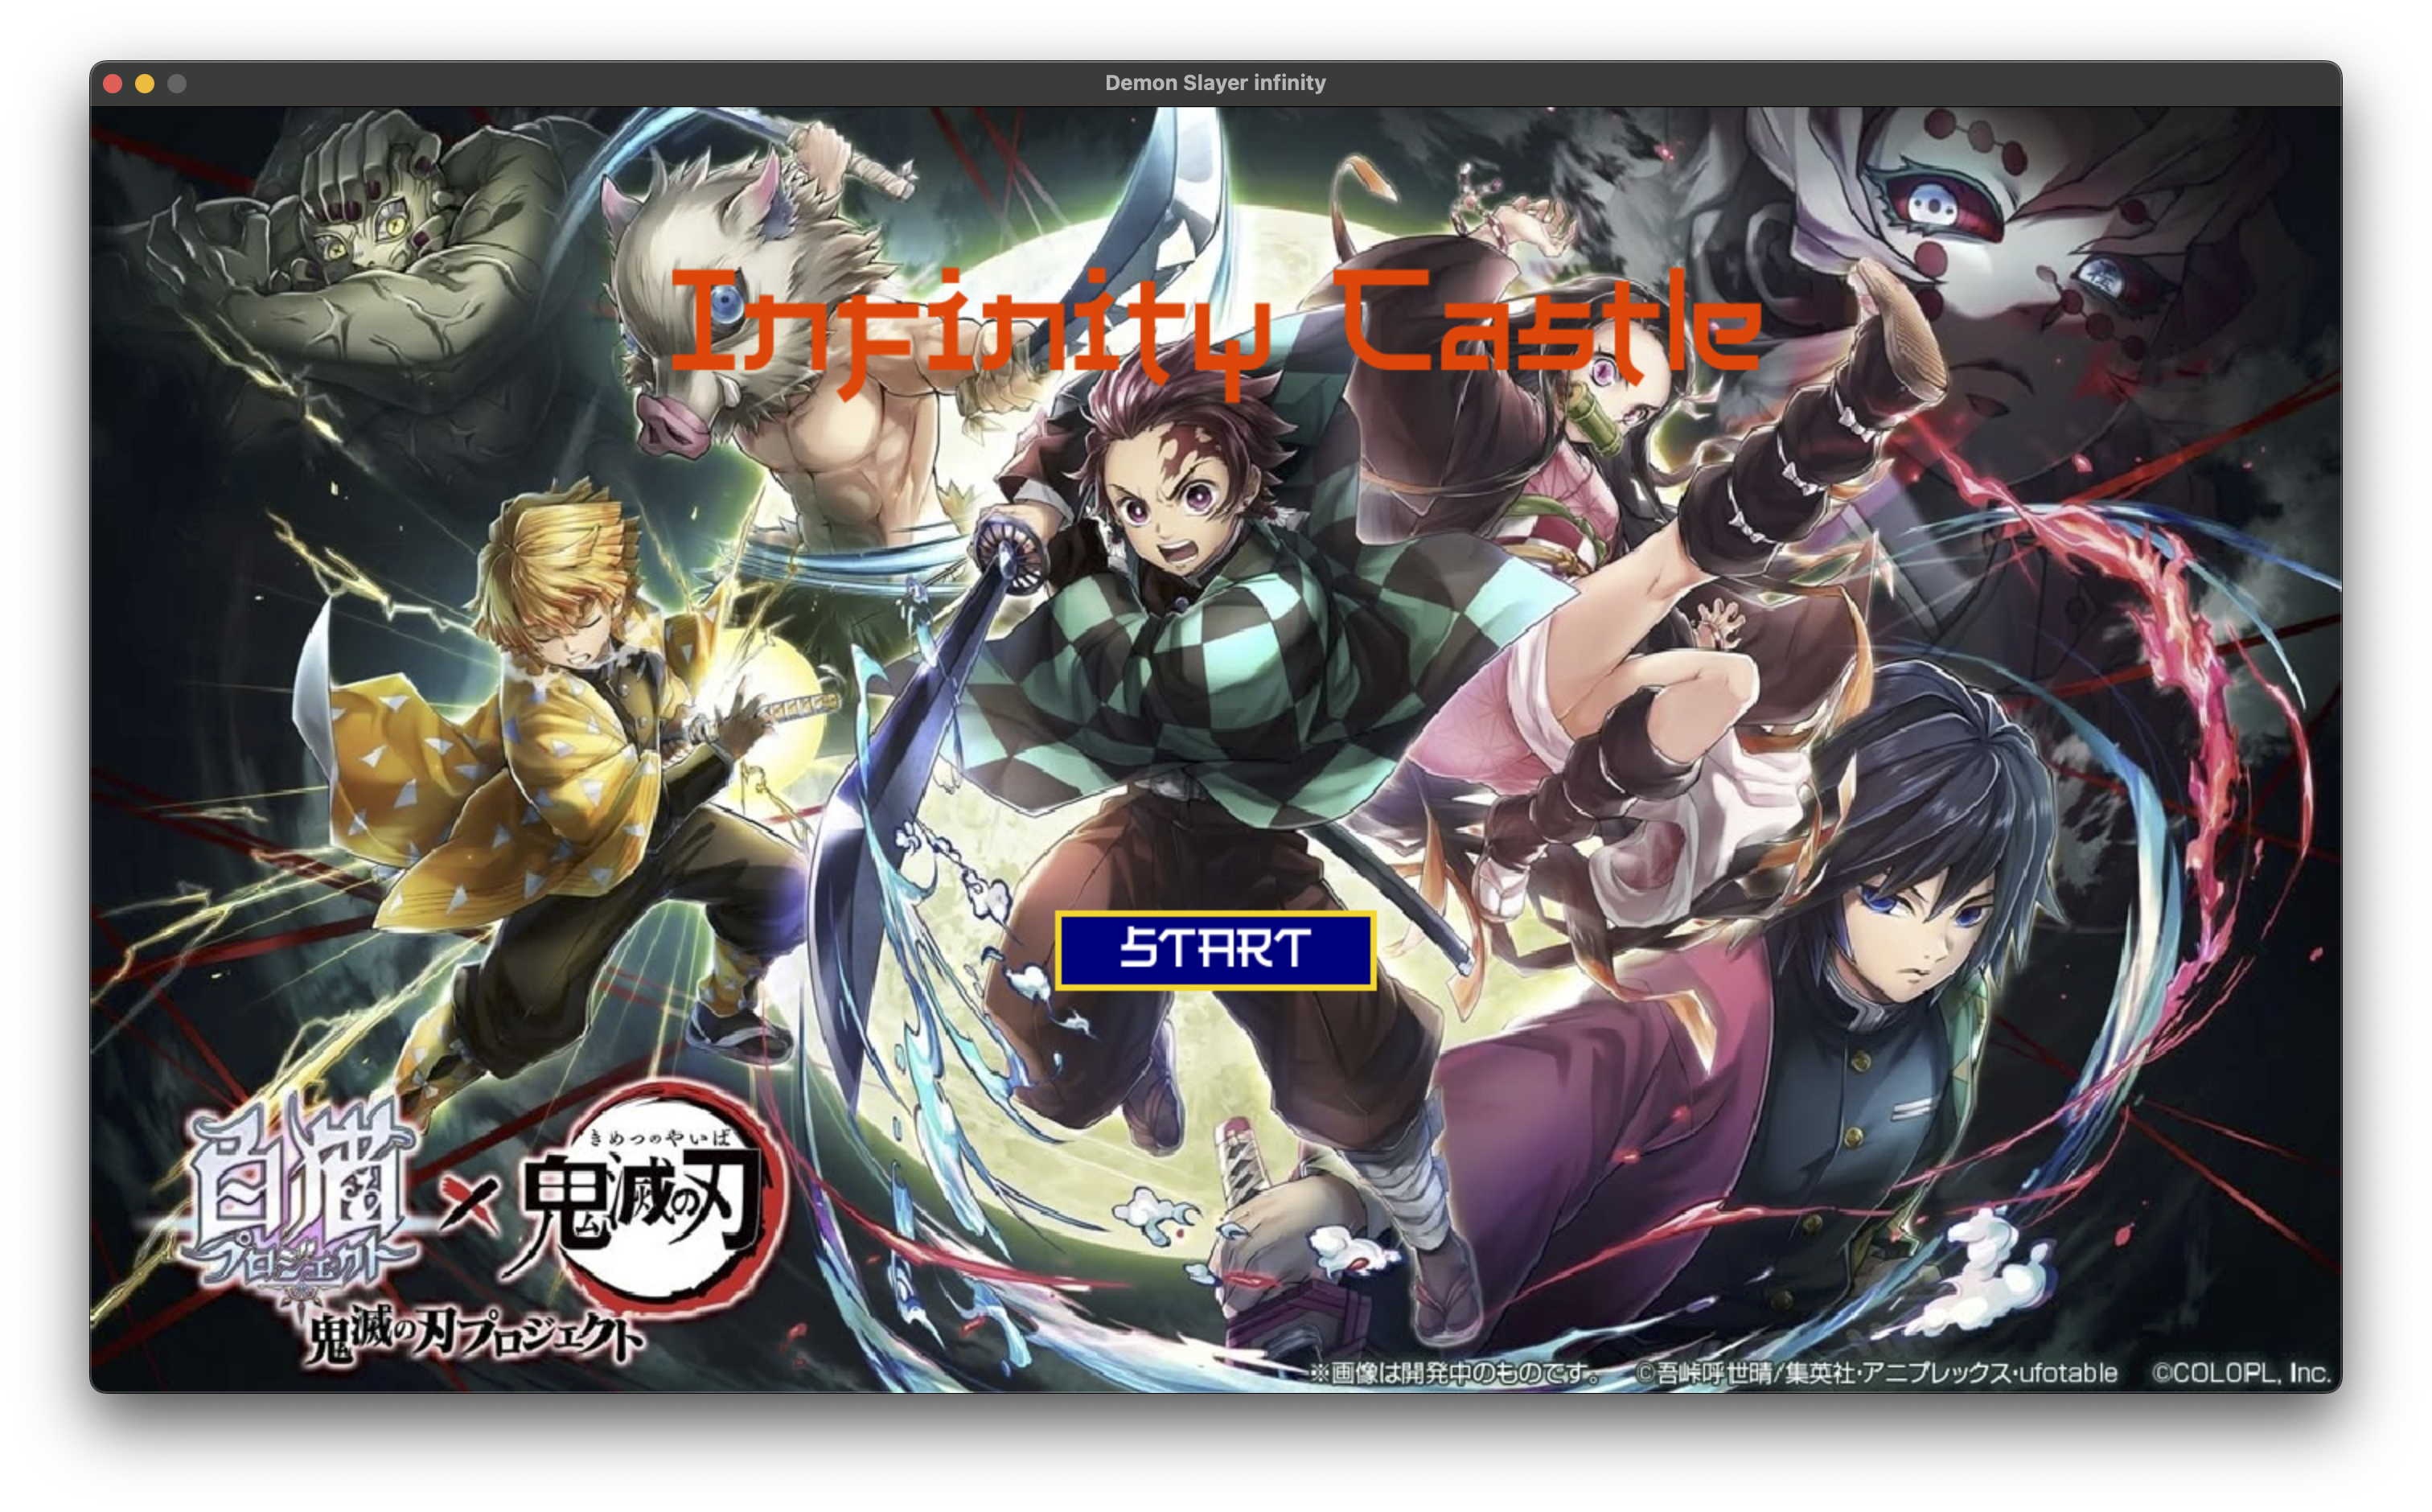
\includegraphics[width=0.5\textwidth]{start_latex}
    \caption{Start screen}
    \label{fig:start}
\end{figure}

\begin{itemize}
    \item Click on the start button to start the game (Figure \ref{fig:start})
\end{itemize}

\begin{figure}[H]
    \centering
    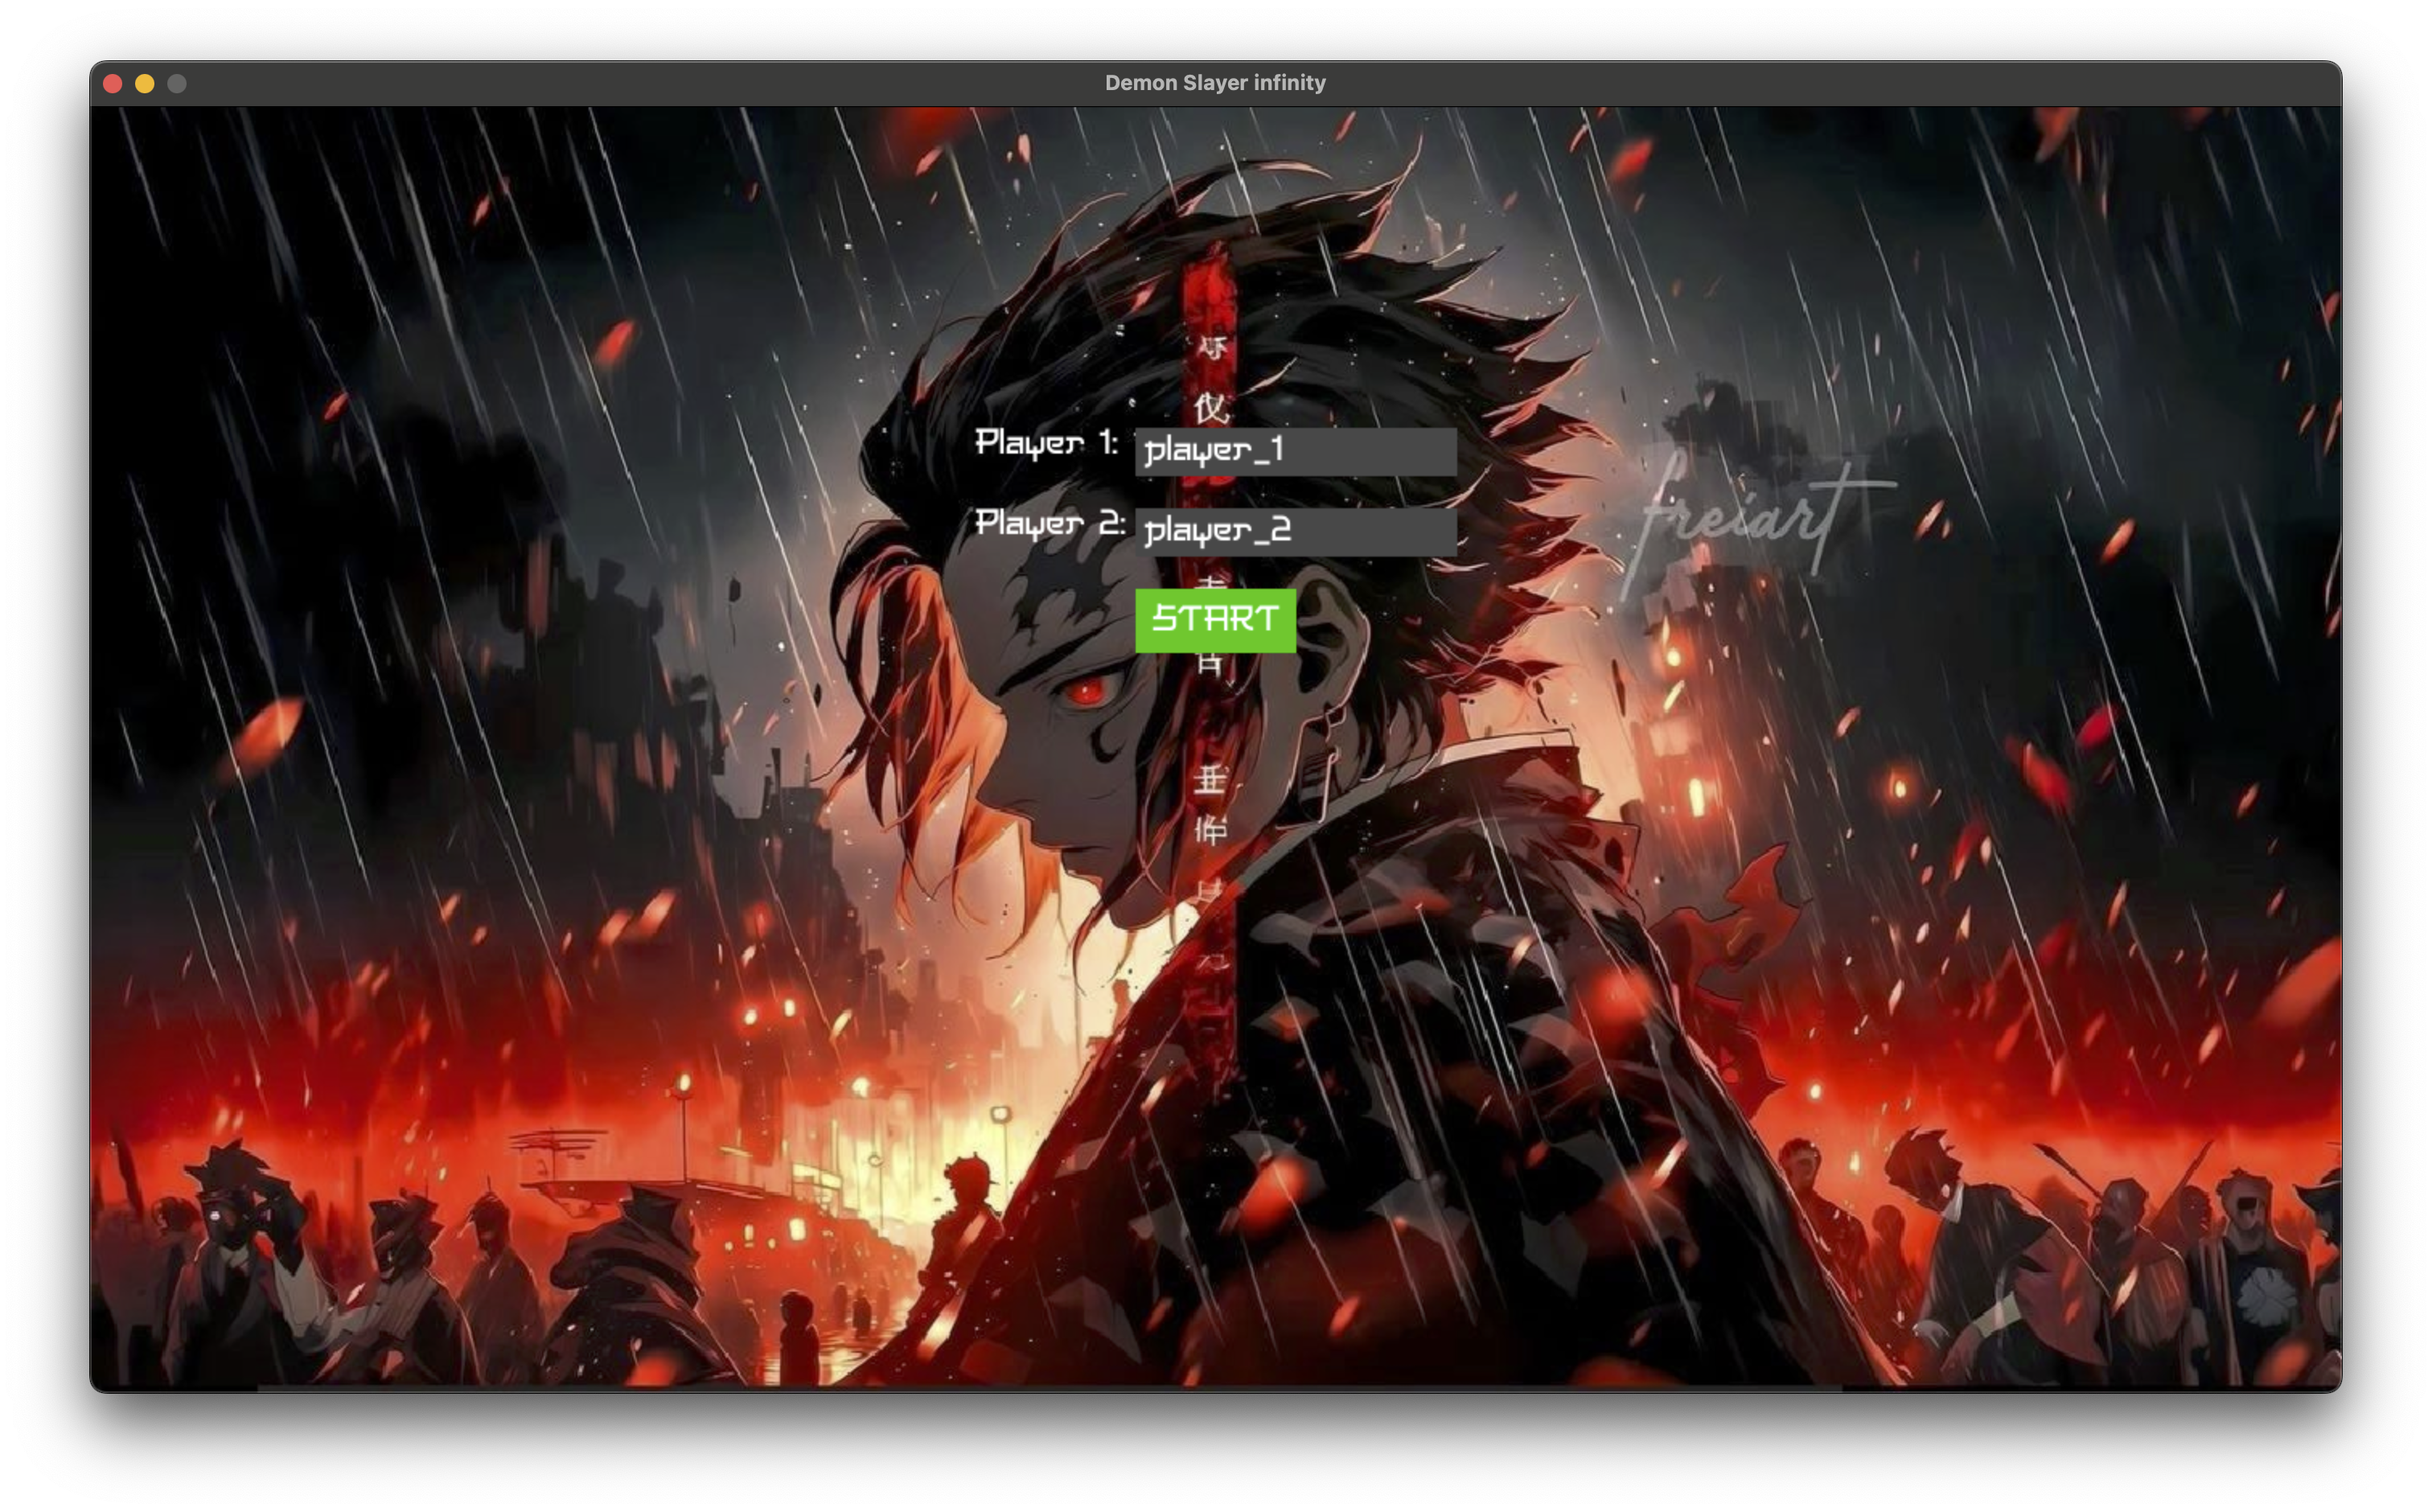
\includegraphics[width=0.5\textwidth]{playerinput_latex}
    \caption{Main menu}
    \label{fig:main_menu}
\end{figure}

\begin{itemize}
    \item Now you can enter your names and hit the start button to select the characters of your choice (Figure \ref{fig:main_menu})
\end{itemize}

\begin{figure}[H]
    \centering
    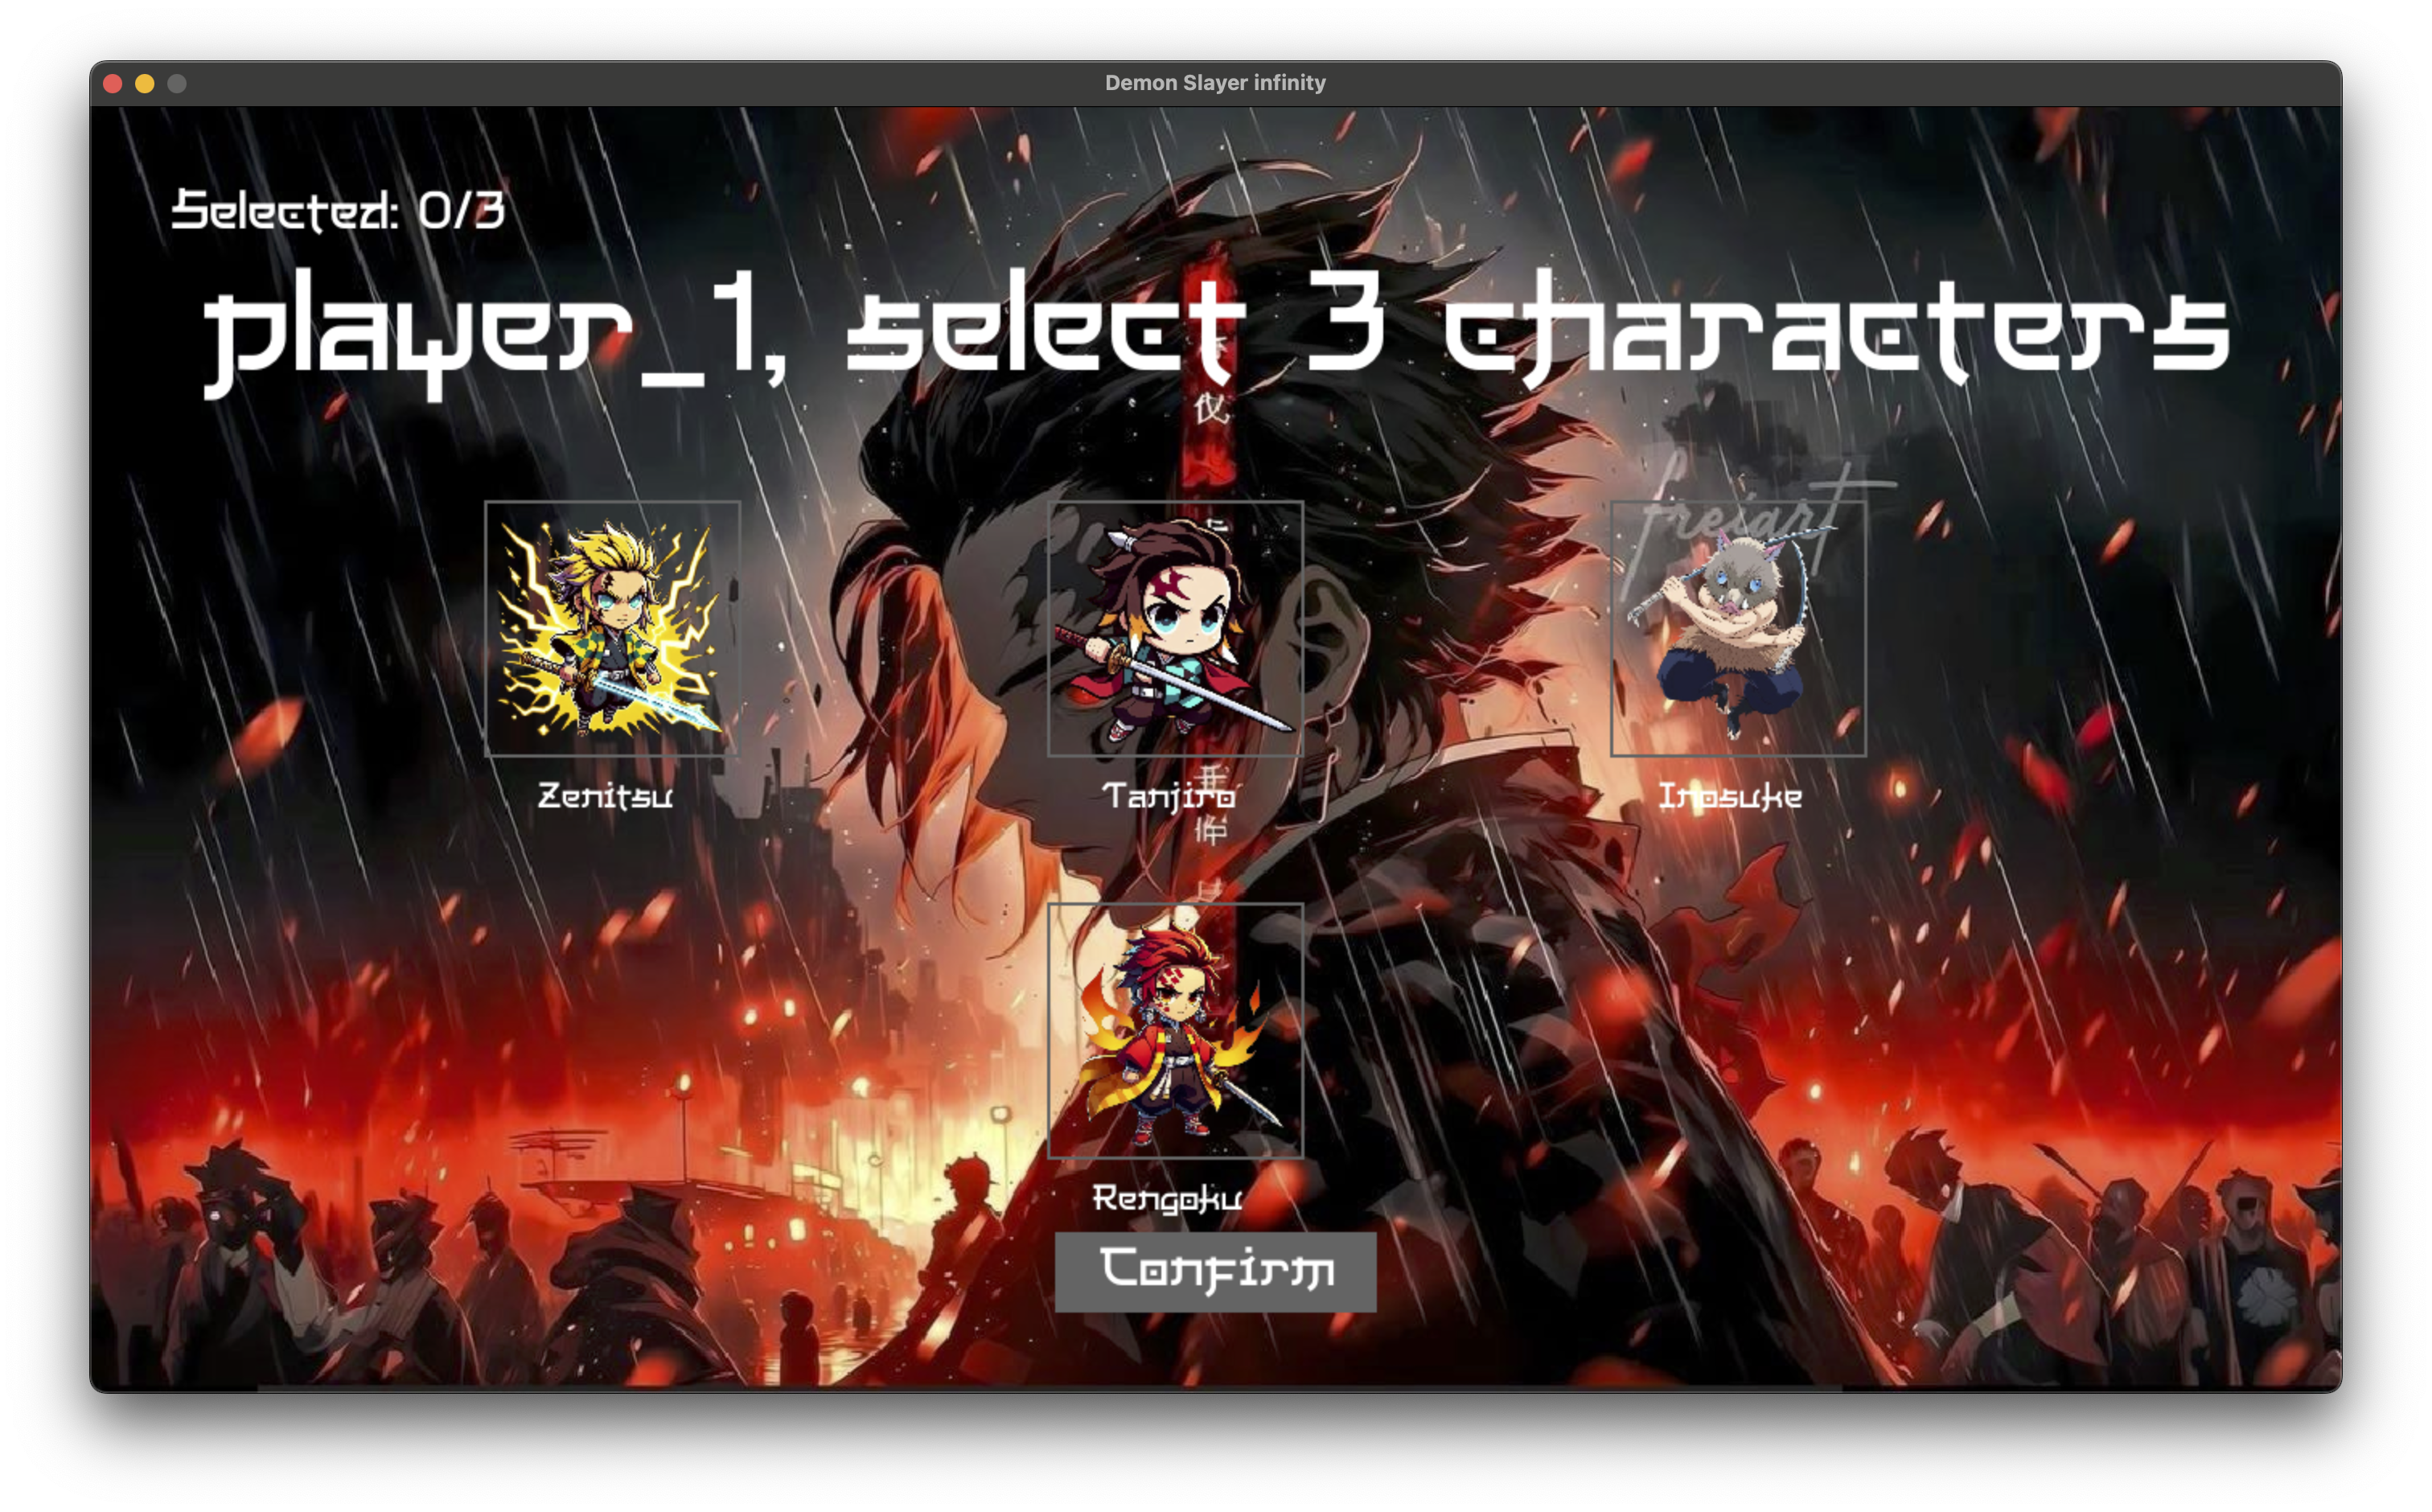
\includegraphics[width=0.5\textwidth]{charselection_latex}
    \caption{Character selection screen}
    \label{fig:character_selection}
\end{figure}

\begin{itemize}
    \item On screen you can select three characters out of 4 characters for each player (Figure \ref{fig:character_selection})
    \item Please select characters carefully as each has different abilities and makes different damage to the different blocks
    \item Rengoku will damage all the blocks equally 
    \item Tanjiro will damage the block type-ice more than the other blocks 
    \item Zenitsu will damage the block type-wood more than the other blocks
    \item Inosuke will damage the block type-stone more than the other blocks
    \item Ice type has health of 25
    \item Wood type has health of 50
    \item Stone type has health of 75 
    \item The blocks are the actual villains in the game and they will take damage based on the character deployed 
    \item Click on the confirm button to confirm your selection and start your game 
\end{itemize}

\begin{figure}[H]
    \centering
    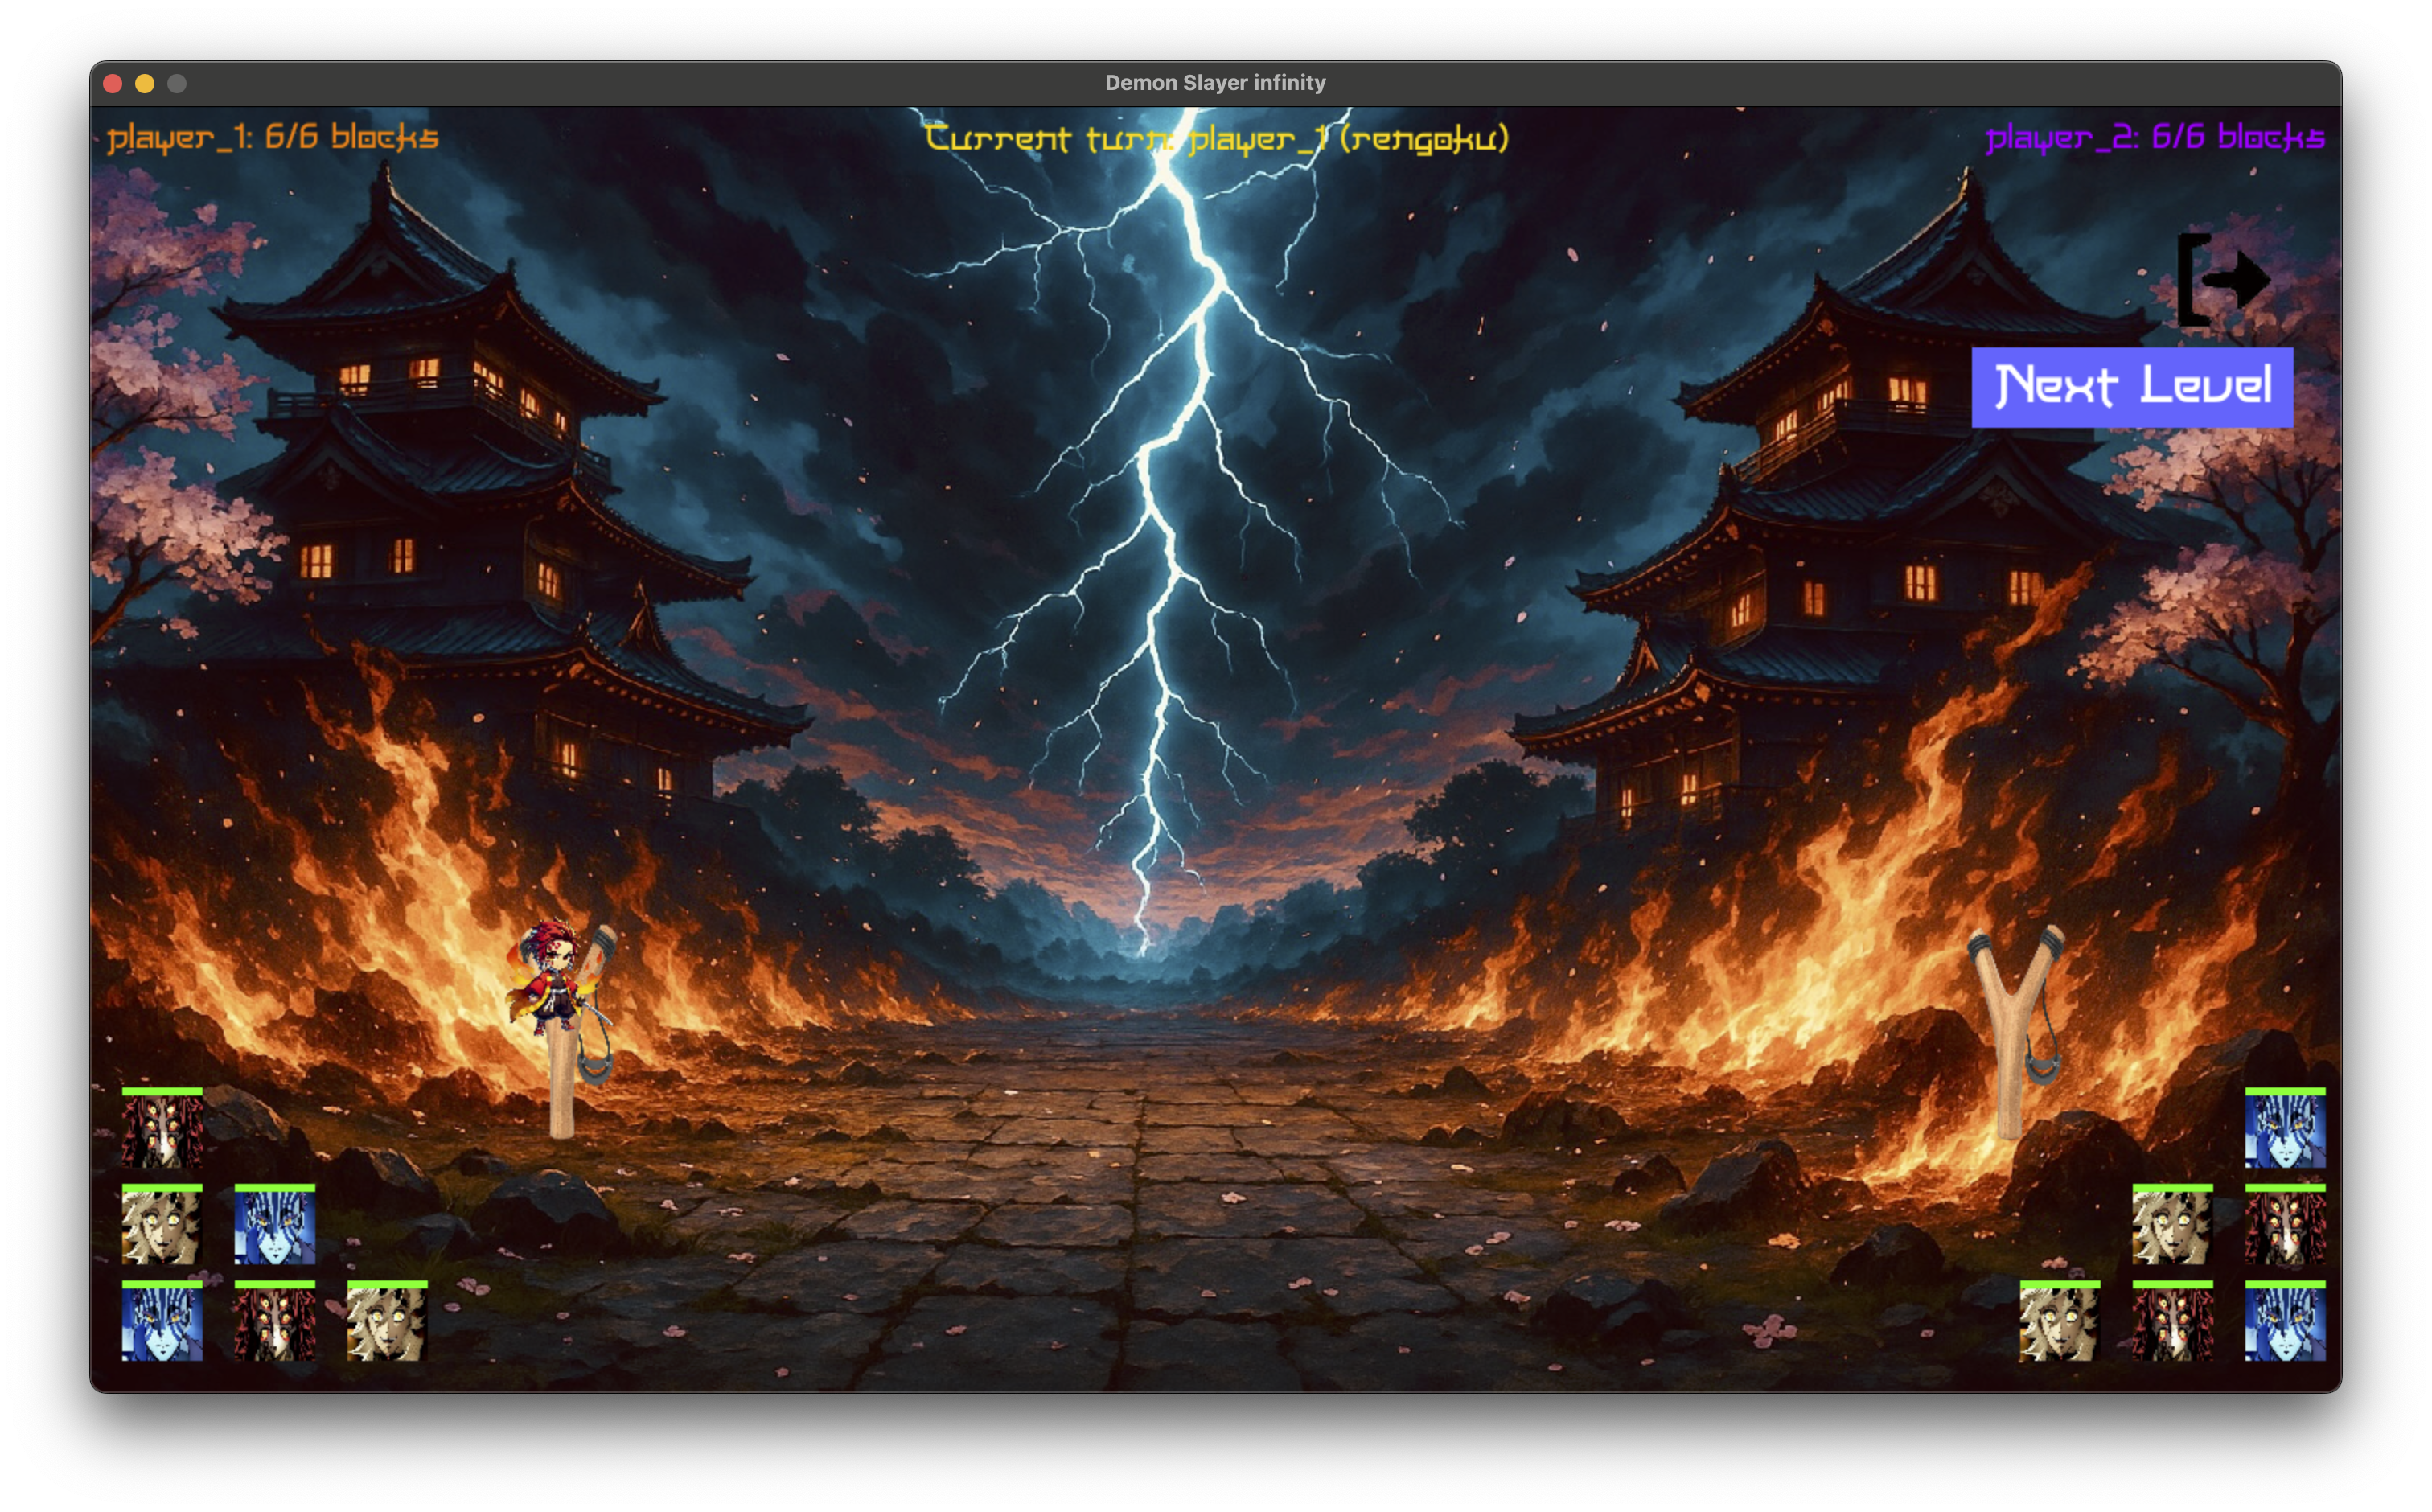
\includegraphics[width=0.5\textwidth]{playinggame_latex}
    \caption{Playing the game}
    \label{fig:playing_game}
\end{figure}

\begin{itemize}
    \item The game will start and you can play the game using the mouse
    \item Place the mouse on the characters and drag the characters to deploy them. When hitting the blocks, blocks take damage based on the character deployed (Figure \ref{fig:playing_game})
    \item The game will end when all the blocks are destroyed or all the characters are deployed
\end{itemize}

\begin{figure}[H]
    \centering
    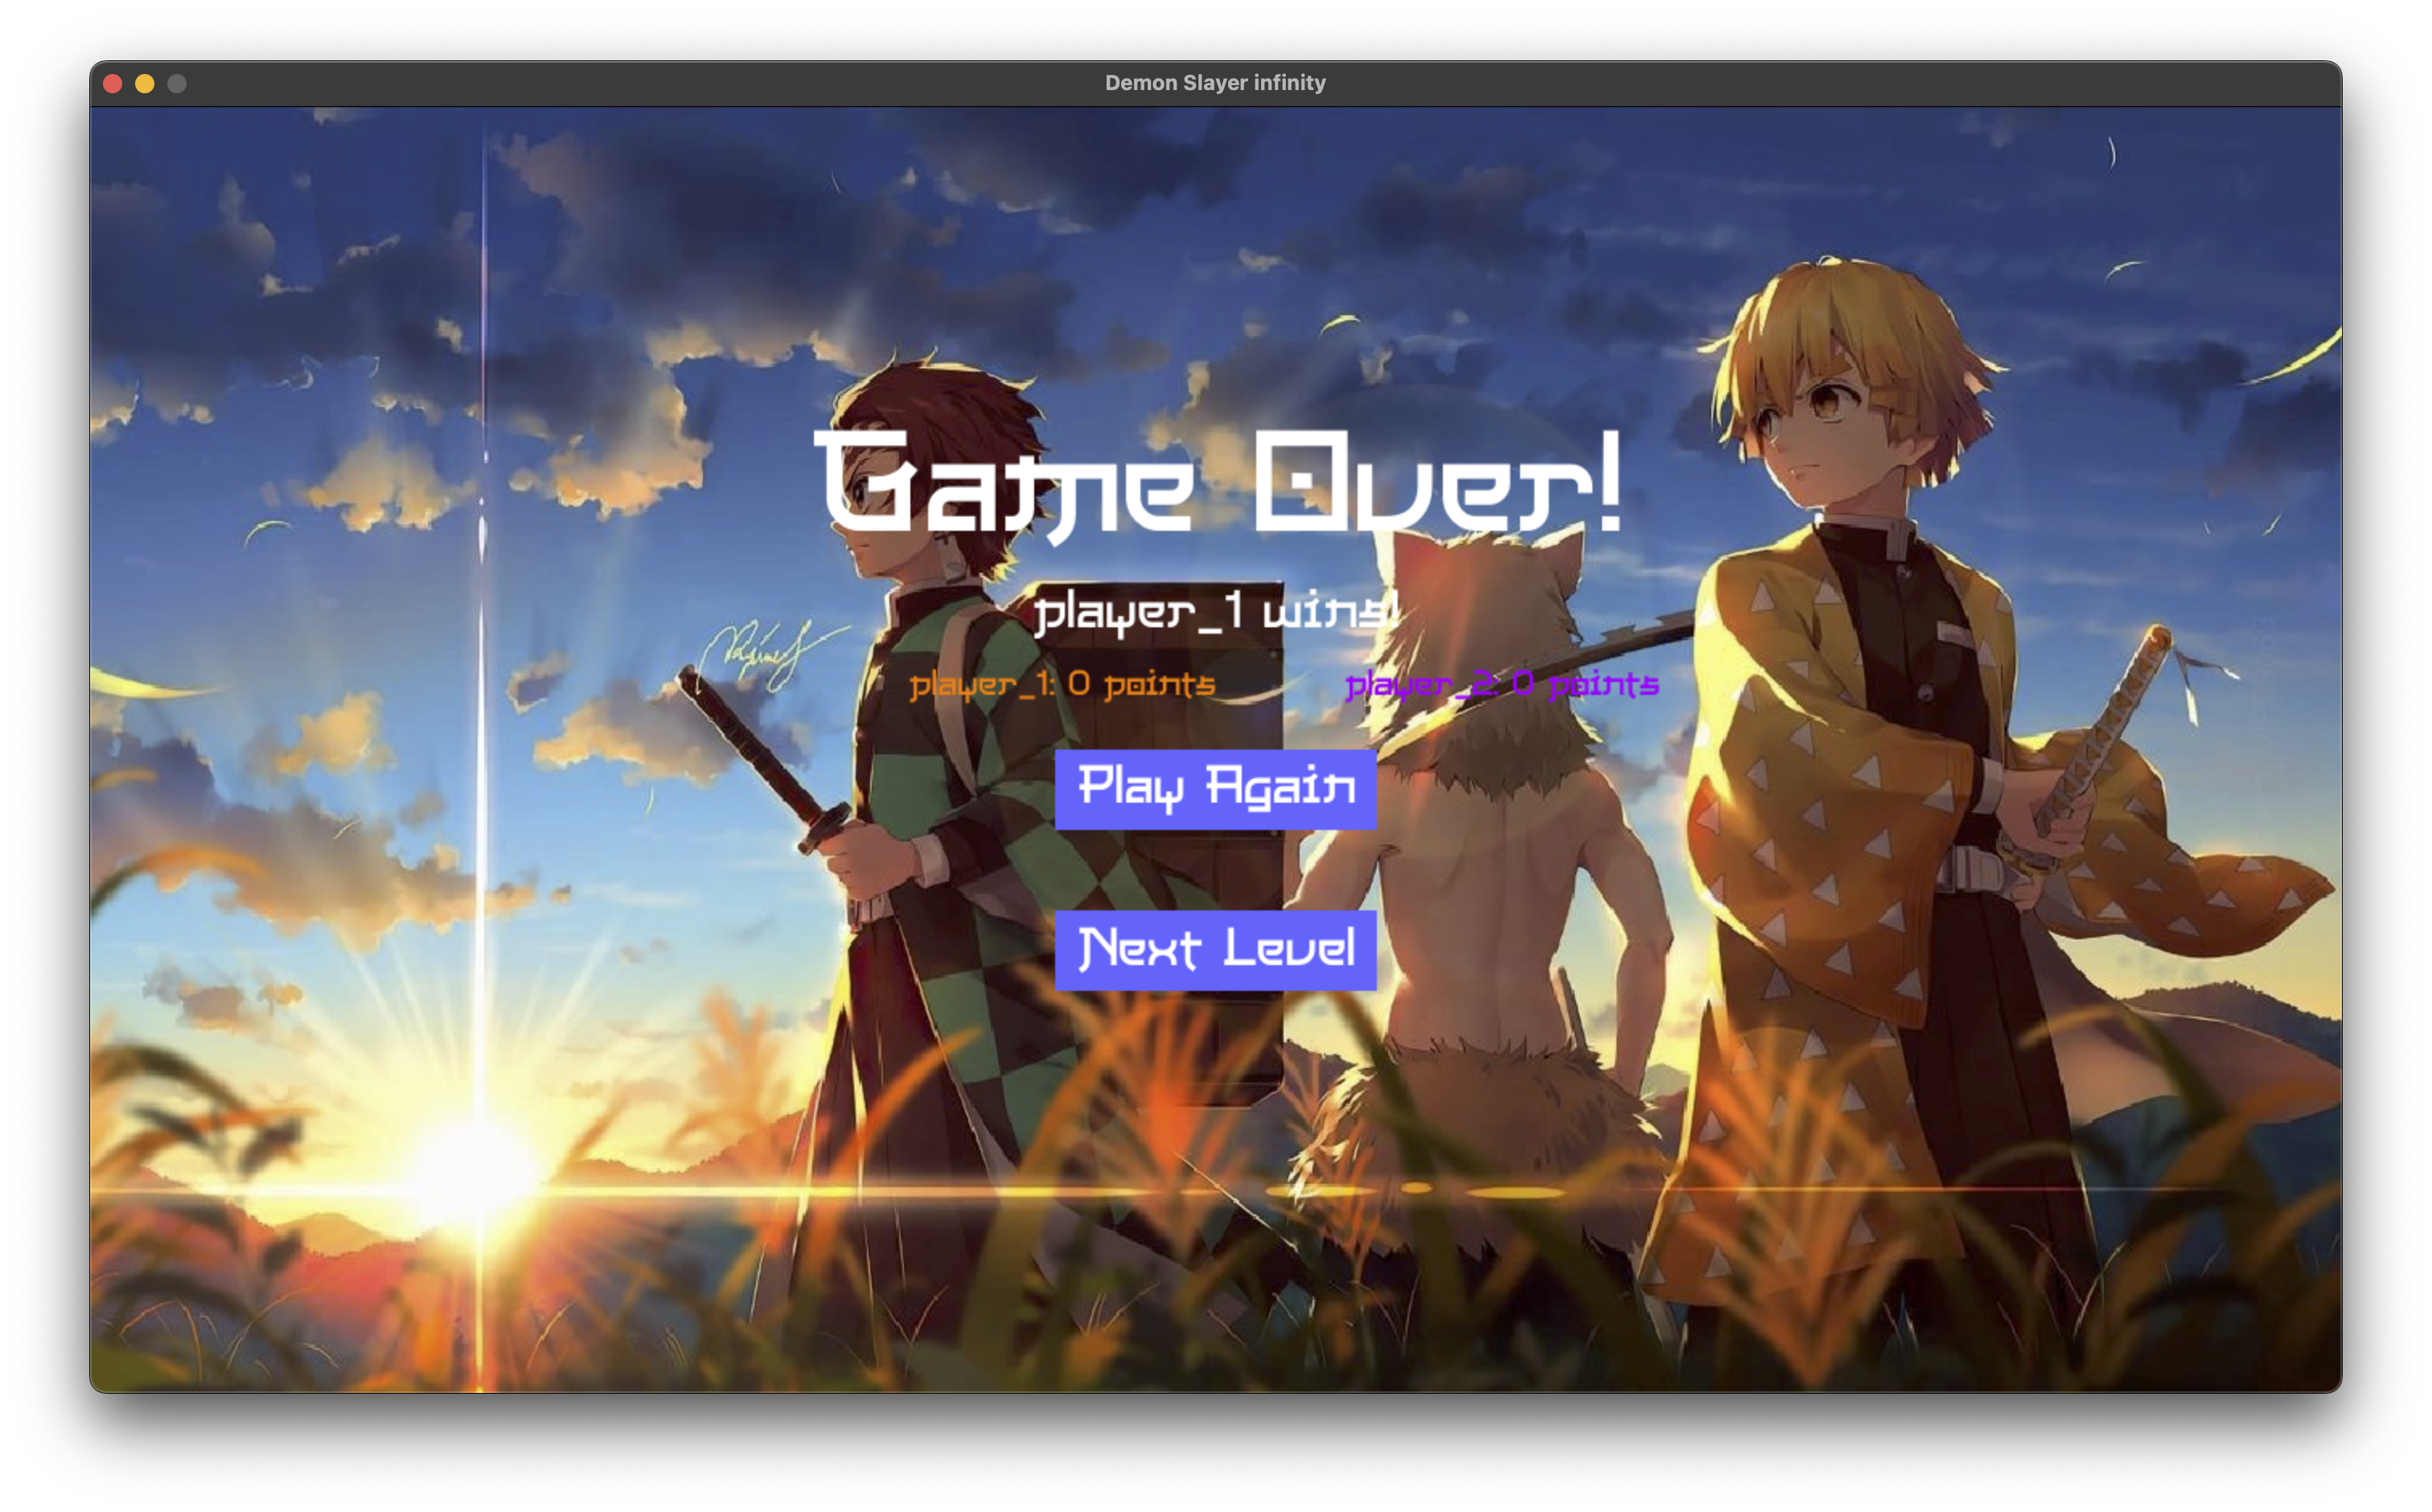
\includegraphics[width=0.5\textwidth]{game_over_latex}
    \caption{Game over screen}
    \label{fig:game_over}
\end{figure}

\begin{itemize}
    \item The game will show the score and the winner of the game. The winner will be decided based on minimum number of characters deployed (Figure \ref{fig:game_over})
    \item Click on the play again button to play the game again
    \item Click on the exit button to exit the game
    \item Click on the next level button to play the next level of the game or you can exit the game 
\end{itemize}

\begin{figure}[H]
    \centering
    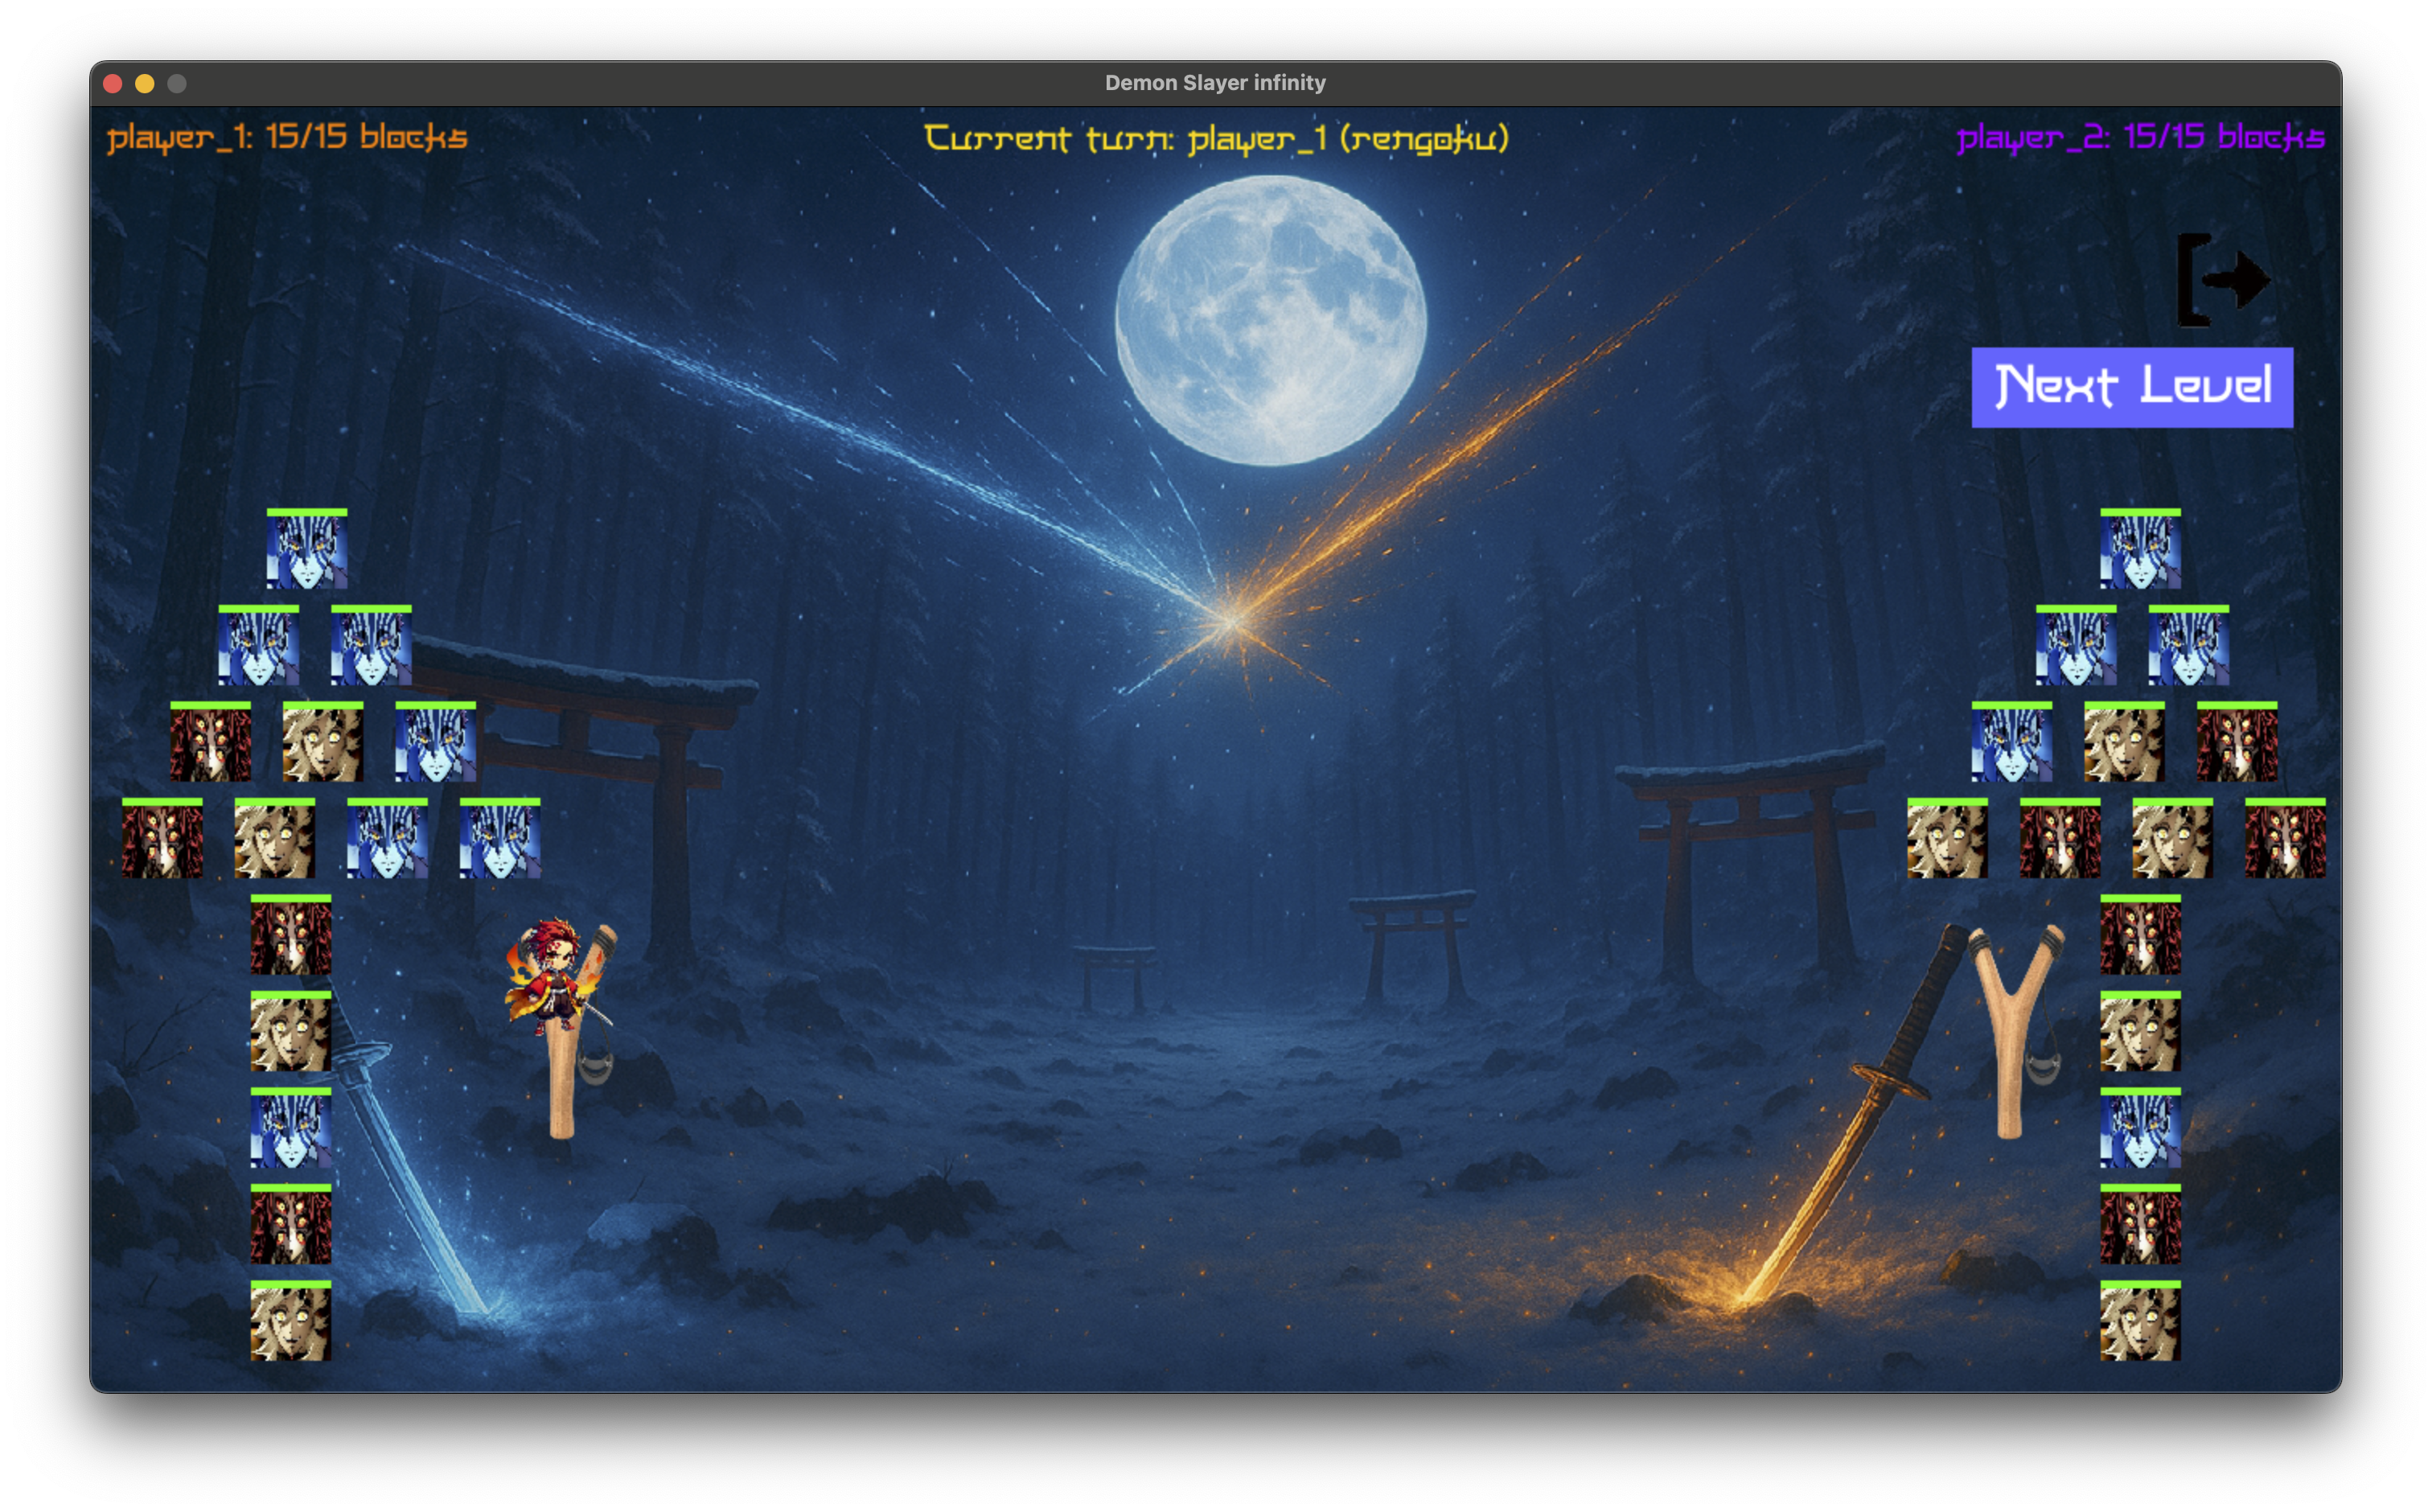
\includegraphics[width=0.5\textwidth]{next_level_latex}
    \caption{Next level screen}
    \label{fig:next_level}
\end{figure}

\subsection{Key features}
\begin{itemize}
    \item Two player game
    \item Each character has its own unique abilities
    \item Each character has its own unique damage
    \item Each block has its own unique health, they are the actual villains in the anime with health allocated based on their hierarchy
    \item To increase the fun factor I have introduced some special effects for the blocks and characters
    \item Rengoku resembles the fire and is the strongest character in the game
    \item Tanjiro resembles the crimson flame and is the main character in the anime
    \item Zenitsu resembles the thunder and is a friend of Tanjiro
    \item Inosuke resembles the wild boar and is the friend of Tanjiro
    \item There are three villain types in the game
    \item Each character has its own unique sound effects 
\end{itemize}

\section{Project structure}
\subsection{Directory layout}
The project follows a standard directory layout for Python projects. The main files and directories are as follows:

\begin{verbatim}
infinity_castle/
+-- main.py
+-- declare.py
+-- calculations.py
+-- blocks.py
+-- player.py
+-- play.py
+-- set.py
+-- interface.py
+-- images/
|   +-- start.jpg
|   +-- main_menu.jpeg
|   +-- battlefield.jpeg
|   +-- next_level.png
|   +-- game_over.jpeg
|   +-- block1.png
|   +-- block2.png
|   +-- block3.png
|   +-- rengoku.png || rengoku!.png
|   +-- tanjiro.png || tanjiro!.png
|   +-- zenitsu.png || zenitsu!.png
|   +-- inosuke.png || inosuke!.png
|   +-- special_block.png
+-- music/
|   +-- demonslayertheme.mp3
|   +-- playing_ds.mp3
|   +-- game_over_bgm.mp3
|   +-- rengoku_bgm.mp3
|   +-- tanjiro_bgm.mp3
|   +-- zenitsu_bgm.mp3
|   +-- inosuke_bgm.mp3
|   +-- special_hit_bgm.mp3
+-- start.otf
\end{verbatim}

\subsection{File descriptions}
\begin{itemize}
    \item \textbf{main.py}: The main file that runs the game. It initializes the game and starts the main loop.
    \item \textbf{declare.py}: This file contains all the global variables and constants used in the game.
    \item \textbf{calculations.py}: This file contains all the calculations and logic for the game.
    \item \textbf{blocks.py}: This file contains the class for the effects for blocks used in the game.
    \item \textbf{player.py}: This file contains the class for the players used in the game.
    \item \textbf{play.py}: This file contains the class for the game play.
    \item \textbf{set.py}: This file contains all the settings and configurations for the player.
    \item \textbf{interface.py}: This file contains all the interface related code for the game.
    \item \textbf{images/}: This directory contains all the images used in the game.
    \item \textbf{music/}: This directory contains all the music files used in the game.
    \item \textbf{start.otf}: This file contains the font used in the game.
\end{itemize}

\subsection{Module descriptions}
\begin{itemize}
    \item \textbf{pygame}: This module is used for creating the game window and handling the game events.
    \item \textbf{random}: This module is used for generating random numbers.
    \item \textbf{numpy}: This module is used for handling the arrays and matrices.
    \item \textbf{math}: This module is used for handling the mathematical calculations.
\end{itemize}

\section{Class descriptions}
\begin{itemize}
    \item \textbf{ui}: This class is used for handling the user interface of the game. It contains all the methods for drawing the interface and handling the buttons.
        \begin{itemize}
            \item \textbf{\_\_init\_\_}: This method is used for initializing the ui class. It contains fonts required for the game.
            \item \textbf{Methods:}
                \begin{itemize}
                    \item \textbf{draw\_menu}: This method is used for drawing the main menu of game. It contains the start button and background image.
                    \item \textbf{draw\_player\_info}: This method is used for drawing the player information layout on the screen it contains the player name and start button.
                    \item \textbf{take\_input}: This method is used for taking the player input from the user. It contains the text box and the start button.
                    \item \textbf{draw\_character\_selection}: This method is used for drawing the character selection screen. It contains the character images and the confirm button.
                    \item \textbf{draw\_game\_over}: This method is used for drawing the game over screen. It contains the game over image, winner name, scores, play again button and next level button.
                \end{itemize}
        \end{itemize}
    \item \textbf{declare}: This class is used for handling the global variables and constants used in the game. It contains all the global variables and constants used in the game.
        \begin{itemize}
            \item \textbf{\_\_init\_\_}: This method is used for initializing the declare class. It contains all the global variables and constants used in the game.       
        \end{itemize}
    \item \textbf{player}: This class is used for handling the player information and the player actions. It contains all the methods for handling the player actions.    
        \begin{itemize}
            \item \textbf{\_\_init\_\_}: This method is used for initializing the player class. It contains the character type, initial position, position, velocity, wind, etc.
            \item \textbf{Methods:}
                \begin{itemize}
                    \item \textbf{load\_image}: This method is used for loading the character image. It contains the character type and the image path.
                    \item \textbf{start\_drag}: This method is used for starting the drag of the character. It contains the mouse position and the character image.
                    \item \textbf{update\_drag}: This method is used for updating the drag of the character. It contains the mouse position and the character image.
                    \item \textbf{end\_drag}: This method is used for ending the drag of the character. It contains the mouse position and the character image.
                    \item \textbf{update}: This method is used for updating the character position, velocity, wind etc.
                    \item It also contains the methods for drawing trajectory, updating wind particles, creating wind particles.
                \end{itemize}
        \end{itemize}
    \item \textbf{blocks}: This class is used for handling the blocks in the game. It contains all the methods for handling the blocks.
        \begin{itemize}
            \item \textbf{\_\_init\_\_}: This method is used for initializing the blocks class. It contains the block type, initial position, health, etc.
            \item \textbf{Methods:}
                \begin{itemize}
                    \item \textbf{draw\_block}: This method is used for drawing the block on the screen. It consists of block image, position, health, etc. It also used for showing special effects on the block.
                    \item \textbf{draw\_health\_bar}: This method is used for drawing the health bar of the block. It contains the block image, position, health, etc.
                    \item I have created many methods in this module to handle the special effects during the game in reaction with collision of character with block.
                    \item I have introduced a special block which will appear randomly while running the game. It has some bonus points. \textbf{SpecialBlock}
                    \item There are many methods I have just included the important ones; the remaining methods are for special effects.
                    \item \textbf{update}: This method is used for updating the block, health, etc.
                \end{itemize}    
        \end{itemize}
    \item \textbf{set}: This class is used for handling player and blocks combinedly. In simple way it links blocks of player.
        \begin{itemize}
            \item \textbf{\_\_init\_\_}: This method is used for initializing the set class. It contains the player blocks, slingshots etc.
            \item \textbf{Methods:}
                \begin{itemize}
                    \item \textbf{add\_block}: This is used to add the blocks to the corresponding player.
                    \item \textbf{initialise\_blocks}: This method is used for loading the images for the game. It contains the image path and type of block.
                    \item \textbf{change\_character}: This method is used for changing the characters randomly after the turn is completed.
                    \item There are some other methods like drawing\_blocks(), is\_castle\_destroyed(), draw\_slingshot() etc.
                \end{itemize}
        \end{itemize}    
    \item \textbf{play}: This class is used for handling the game play, music and deciding winner etc.
        \begin{itemize}
            \item \textbf{\_\_init\_\_}: This method is used for initializing the play class. It contains the player blocks, slingshots, game state music etc.
            \item \textbf{Methods:}
                \begin{itemize}
                    \item \textbf{play\_background\_music}: This method is used for playing the background music. It contains the music path and volume.
                    \item \textbf{handle\_events}: This method is used for handling the events of the game like mouse button down, mouse button up, mouse motion etc.
                    \item \textbf{update}: This method is used for updating the game state. It contains the game state and player blocks.
                    \item \textbf{draw}: This method is used for drawing the game on the screen. It contains the game state and player blocks.
                    \item There are some other methods like run(), draw\_game\_over() etc.
                \end{itemize}
        \end{itemize}    
    \item There are some other classes like \textbf{calculations}, \textbf{main} etc. which are used for handling the calculations and main game startup.     
\end{itemize}

\section{Technical implementation}
\subsection{Game loop}
The game loop is the main loop of the game. It runs continuously until the game is over. The game loop handles all the events and updates the game state. The game loop is implemented in the main.py file. The main loop is as follows:

\begin{verbatim}
def run(self):
    if self.game_state == "menu":
        self.play_background_music(self.menu_music)
    while self.running:
        if self.current_game_state != self.game_state:
            if self.game_state == "menu":
                self.play_background_music(self.menu_music)
            elif self.game_state == "playing":
                self.play_background_music(self.playing_music)
                pygame.mixer.music.set_volume(0.2)
                self.effect_channel.set_volume(1.0)
            elif self.game_state == "game_over":
                self.play_background_music(self.game_over_music)
            self.current_game_state = self.game_state
        self.handle_events()
        self.update()
        self.draw()
        self.dt = self.timer/ 1000
        self.timer = self.clock.tick(60)
    pygame.quit()
    sys.exit()
\end{verbatim}

\subsection{Event handling}
The event handling is done in the handle\_events() method. The event handling is done using the pygame library.
In handle\_events() method we handle the events of the game. There are different handling methods inside the handle\_events() method
like handling\_menu\_events(), handling\_playing\_events(), handling\_game\_over\_events() etc.
For example: handling\_playing\_events() method is as follows:

\begin{verbatim}
def handle_playing_events(self, event):
    """Handle events during gameplay"""
    current_player = self.players[self.current_player_idx]
    player_x = current_player.player_x
    
    if event.type == pygame.MOUSEBUTTONDOWN:
        if event.button == 1 and not player_x.is_thrown:  # Left mouse button
            mouse_pos = pygame.Vector2(event.pos)
            player_x.start_drag(mouse_pos)
            exit_button = self.ui.draw_exit(self.screen)
            if exit_button.collidepoint(event.pos):
                self.game_state = "menu"
                self.background = self.menu_background
                self.current_player_a_blocks = player_a_blocks
                self.current_player_b_blocks = player_b_blocks
    
    elif event.type == pygame.MOUSEMOTION:
        if player_x.is_dragging:
            mouse_pos = pygame.Vector2(event.pos)
            player_x.update_drag(mouse_pos)
    
    elif event.type == pygame.MOUSEBUTTONUP:
        if event.button == 1 and player_x.is_dragging:
            mouse_pos = pygame.Vector2(event.pos)
            player_x.end_drag(mouse_pos)
\end{verbatim}

Above code is used to handle the events of the game like mouse button down, mouse button up, mouse motion etc, while playing the game 
and also handling the events of the game like exit button.
There are different files for handling all the events of the characters and blocks.

\subsection{Game state management}
The game state management is done using the game\_state variable. The game\_state variable is used to manage the different states of the game. The different states of the game are:
\begin{itemize}
    \item menu: The main menu of the game
    \item playing: The game is being played
    \item game\_over: The game is over
    \item next\_level: The next level of the game
\end{itemize}

\section{Basic features}
\subsection{Game interface}
Developed a UI with a main menu and enter the players names before starting the main game. The start of the game will take you to the gameplay screen.
Some music was added to it to get the feel of Demon Slayer anime.

\subsection{2-Player Gameplay}
Players launch projectiles competing to destroy structures. Turn-based gameplay.
The deployable characters will be generated randomly based on selection of characters.

\subsection{Projectile mechanics}
Implemented a gravity-based launching system where players use mouse input (drag and pull) to control the angle and force.

\subsection{Game Over Conditions}
Define winning and losing conditions based on destroying the opponent structure/fort to an extent/entirely.

\subsection{Projectile effects}
Each character has unique abilities towards the different blocks.

\begin{verbatim}
"zenitsu": {
    "image": "images/zenitsu!.png",
    "damage_multiplier": {"wood": 1.0, "ice": 0.8, "stone": 0.8},
     "song" : "music/zenitsu_bgm.mp3"
},
"tanjiro": {
    "image": "images/tanjiro!.png",
    "damage_multiplier": {"wood": 0.8, "ice": 1.0, "stone": 0.8},
    "song" :"music/tanjiro_bgm.mp3"
},
"inosuke": {
    "image": "images/inosuke.png",
    "damage_multiplier": {"wood": 0.8, "ice": 0.8, "stone": 1.0},
    "song" :"music/inosuke_bgm.mp3"
},
"rengoku": {
    "image": "images/rengoku!.png",
    "damage_multiplier": {"wood": 1, "ice": 1, "stone": 1},
    "song" : "music/rengoku_bgm.mp3"
}
\end{verbatim}

\section{Advanced features}
\subsection{Sound effects}
Added sound effects: background music for different states, character-specific sounds for launching projectiles, and block special block hit sounds.

\subsection{Game Level}
The game has two levels. The first level is the main game and the second level has more blocks and a different background.

\subsection{Custom Theme for the game}
The game has a custom theme based on the anime "Demon Slayer". The characters and blocks are designed based on the anime characters. The game has a custom font and background music based on the anime.

\subsection{Dynamic Terrain}
Introduced elements like wind and moving obstacles for the bonus points.

\subsection{Scoring System}
Assigned scores based on the number of throws required to destroy the blocks. It defines the art of attacking multiple blocks at time and gives bonus points for doing so within some throws.

\subsection{Destructable elements}
As the blocks are here the main villains in the anime, I didn't want to change their expressions or so and I didn't find some solid images for blocks to change when hit by characters.
So I thought to draw a health bar for the blocks to show the destruction of blocks (villains).

\subsection{Special effects}
I have added some special effects to the blocks and characters. The special effects are based on the anime characters.
\begin{itemize}
    \item For Rengoku I have added fire effects; mixture of red and yellow colored circles of different sizes will be generated.
    \item For Tanjiro I have added a crimson flame effect; mixture of red colored circles of different sizes will be generated.
    \item For Zenitsu I have added a thunder effect; mixture of blue and white circles and lines of different sizes will be generated.
    \item For Inosuke I have added a wild boar effect; mixture of brown colored circles of different sizes will be generated.
    \item For depicting various effects I have used the health bar, here the health bar won't change suddenly, but it will decrease gradually.
\end{itemize}
\begin{figure}[H]
    \centering
    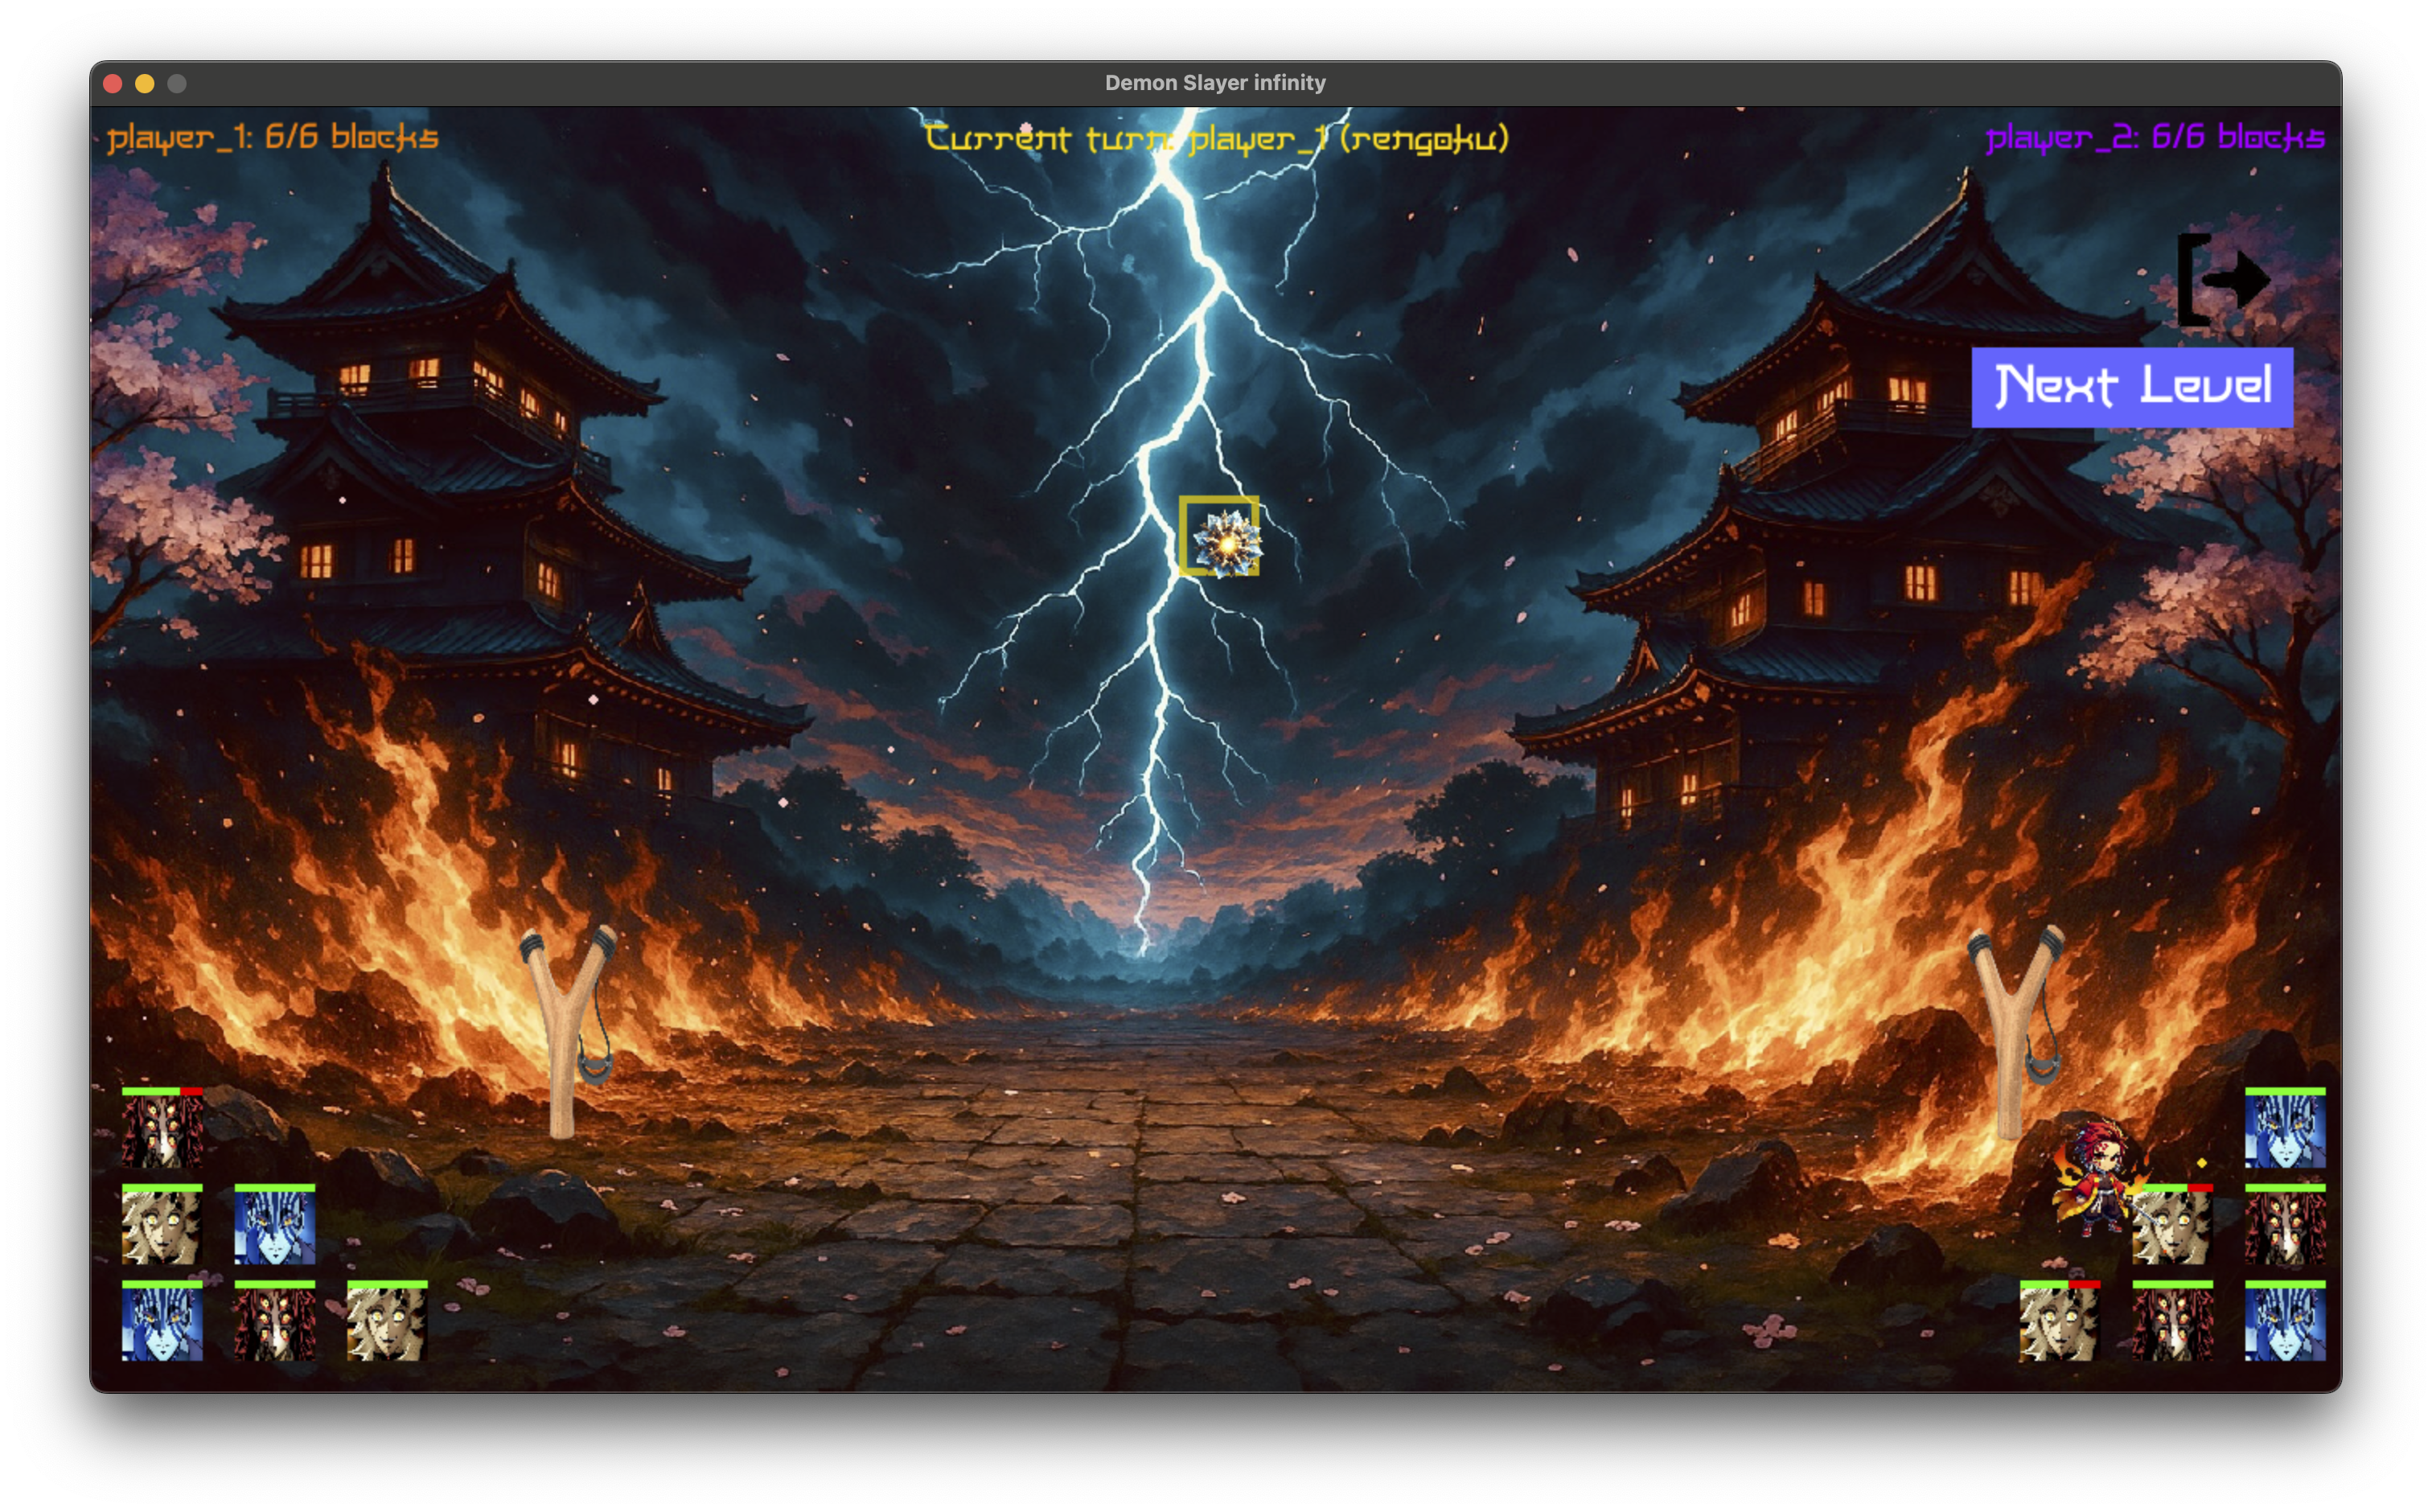
\includegraphics[width=0.5\textwidth]{special_latex}
    \caption{special effects}
    \label{fig:special_effects}
\end{figure}
\textbf{Learnings}
\begin{itemize}
    \item I have learned a lot of things from this project. I have learned how to use the Pygame module and how to handle the events in the game.
    \item I have learned how to create a game with sound effects and music.
    \item I have learned how to create a game with special effects and animations.
    \item The main thing I learned is how to handle a large codebase, organize the code in different files and modules, and be patient while debugging errors.
    \item our brain is better than the AI for some cases, like debugging the code and handling the errors.
\end{itemize}   
\section{Project journey}
I choose this project beacuse, I used to like the demon slayer anime and I wanted to create a game based on it. I started learning the Pygame module and I found it interesting. I started creating the game and I faced many challenges in the beginning. I started with the basic game and then I added the features one by one. I faced many challenges in the beginning like handling the events, creating the game loop, etc. But I learned a lot from these challenges and I enjoyed the process of learning.
\begin{itemize}
    \item I started with the basic version of the game which consists of only single player and no special effects ,and with out any interface or organisation of code.
    \item First I learnt ,hoe to control the mouse events to drag and leave the characters. from pygame documentation.\cite{pygame}
    \item I referred the code organisation and structure from the git hub refeference.\cite{github}
    \item I started with the basic version of the game which consists of only single player and no special effects ,and with out any interface or organisation of code.
    \item I have used git hub copilot auto fill feature to autofill the code and I have used the chapgpt to verify my errors,
    \item I was bad at handling corner cases and I used to get errors like index out of range, list index out of range, etc. I used to get frustrated with these errors and I used to spend a lot of time debugging the code.
    \item I have used stackoverflow to get the solutions and examples for the functions and methods I used in the code.\cite{stackoverflow}
    \item Stackoverflow is a great platform to get the solutions for the errors and I have used it a lot in this project.
    \item I struggled a lot for finding images for the characters and blocks. I have used the images from internet and some of them are ai generated.
    \item I learnt insertion of music from stackoverflow and I got some issues with the background music and character music , I took help of chatgpt to resolve this problem.It solved it using channels I didn't understand fully but I used it directly.
    \item I took help of chatgpt to resolve the issues with the special effects , and with colour codes.
    \item I took help help of chatgpt to create draw trajectory lighting effect 
    \item In this project, I learned a lot of things about pygame. Surfaces are the main
    things that I took time on. At that, I was very slow but over time I got used to it. This project
    made me increase my patience. I got to know some meaning about debugging in the process. But
    creating a game was a very nice experience for me.
    \item \textbf{Finally I have created a game which is based on the anime Demon Slayer and I am happy with the project.}
\end{itemize}
\printbibliography
\end{document}